\documentclass[]{article}
\usepackage{amsmath}
\usepackage{amsfonts}
\usepackage{amssymb}
\usepackage[utf8]{inputenc}
\usepackage{graphicx}
\usepackage{geometry}
\usepackage{color}
\usepackage{siunitx} %\SI{44.9}{\celsius}
\usepackage[german]{babel}
%\usepackage{circuitikz} für Stromkreise
\long\def \/*#1*/{} %Kommentare mit \/* ---- */
\geometry{
	a4paper,
	left=25mm,
	right=25mm,
	top=25mm,
	bottom=25mm,
}
\pagenumbering{arabic}

\title{Messung der Dampfdruckkurve von Wasser}
\author{Máté Farkas, Patrick Schillings}
\begin{document}
	\begin{center}
		\part*{Versuchsbericht}
		\newpage
	\end{center}
\tableofcontents
\section{Versuchsziele}
Ziel des Versuchs war es durch die Messung der Dampfdruckkurve von Wasser, also den Druck in Abhängigkeit von der Temperatur während der Abkühlphase bei festem Volumen, die molare Verdampfungsenthalpie von Wasser zu bestimmen. Der Dampfdruck ist ein Gleichgewichtsdruck, der sich einstellt, wenn sowohl die flüssige Phase, als auch die gasförmige Phase im Gleichgewicht sind bei hinreichender Größe des Volumens. Die molare Verdampfungsenthalpie ist die Wärme, die ein Mol Flüssigkeit aufnimmt, um in die Gasphase übergehen zu können, und wird auch latente Wärme genannt.
\section{Theoretische Grundlagen}
Hintergrund ist die Clausius-Clapeyron-Gleichung, die aus den ersten beiden Hauptsätzen der Thermodynamik folgt.
Der erste Hauptsatz behandelt dabei die Energieerhaltung:
\begin{equation}
	\Delta U =\Delta Q +\Delta W
	\label{e1}
\end{equation}

Der zweite die Umwandelbarkeit von verschiedenen Energieformen ineinander, was oft mit Hilfe der Entropie formuliert wird:
\begin{equation} 
 	 \Delta S=\frac{\Delta Q_{rev}}{T} \ge 0
 	 \label{e2}
 \end{equation}
Daraus folgt für einen infinitesimalen Prozess entlang der Grenzkurve:
Mit \ref{e1} folgt, wobei $V_1$ das Volumen des Gases ist, $V_2$ das der flüssigen Phase und C die molare Wärmekapazität
\begin{equation} 
 	 \nu((C_{m2}-C_{m1})dT+\frac{d\Lambda}{dT}dT)=dp(V_1-V_2)
 	 \label{e3} 
 \end{equation}
Und weiter mit \ref{e2}
\begin{equation} 
	(C_{m2}-C_{m1})dT+\frac{d\Lambda}{dT}dT-\Lambda\frac{dT}{T}
	\label{e4}
\end{equation}
Bis schließlich die Clausius-Clapeyron-Gleichung
\begin{equation} 
 	 \frac{dp}{dt}=\frac{\nu\Lambda}{T(V_1-V_2)} 
 \end{equation} aus \ref{e3} und \ref{e4} folgt.
Daraus kann man durch Integrieren einen Zusammenhang zwischen dem Druck p und der Temperatur T herauslesen, der über Naturkonstanten und die molare Verdampfungsenthalpie $\Lambda$ gegeben ist:
\begin{equation}
	ln(\frac{p}{p_0})=-\frac{\Lambda}{R}(\frac{1}{T}-\frac{1}{T_0})
\end{equation}
Mit der idealen Gasgleichung $pV=\nu RT$ und der Gaskonstanten R.
\section{Versuchsaufbau}
Ein Rundkolben, der an einem Stativ befestigt ist, befindet sich über einem mit einem Laborheber in der Höhe einstellbaren Heizpilz. Der Kolben hat einen abgedichteten Einlass für den Temperatursensor und oben wird mit dichten Schläuchen ein Drucksensor (Absolutdrucksensor S (524065)) angebracht und ebenso die Zuleitung zu einem Dreiwegehahn gelegt, von dem ein weiteres Ende mit einer Handpumpe verbunden wird. Ein Ausgang ist mit der Umgebung verbunden (vgl. Abb. \ref{Aufbau}).
\begin{figure}
	\begin{center}
		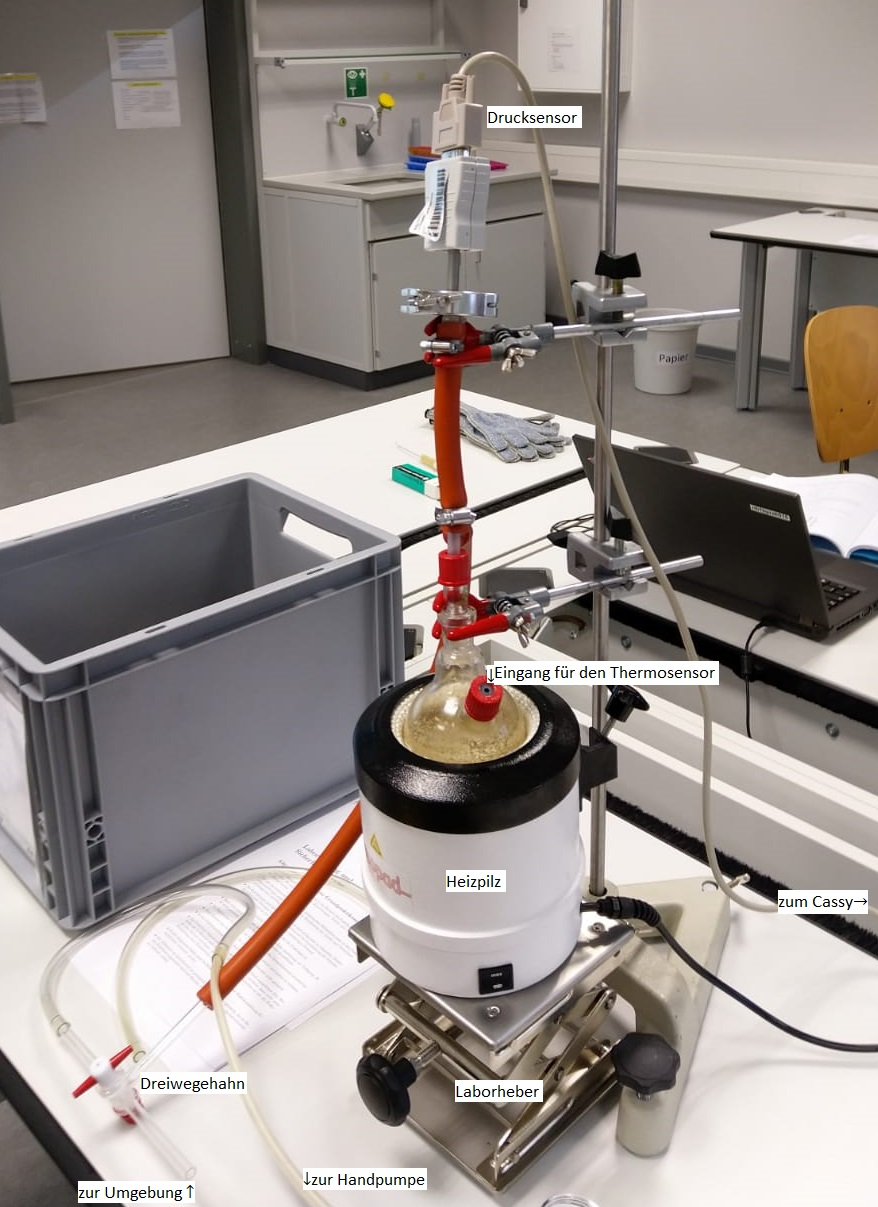
\includegraphics[scale=0.85]{Images/Aufbau.jpg}
		\label{Aufbau}
		\caption{Der Versuchsaufbau}
	\end{center}
\end{figure}
Ein Becherglas mit Eiswasser und ein Becherglas mit unbearbeitetem Wasser stehen bereit. Zur Datensammlung und Erstauswertung wird ein Cassy-System mit den zugehörigen Sensoren verwendet (vgl. Abb. \ref{Cassy}).
\begin{figure}
	\begin{center}
		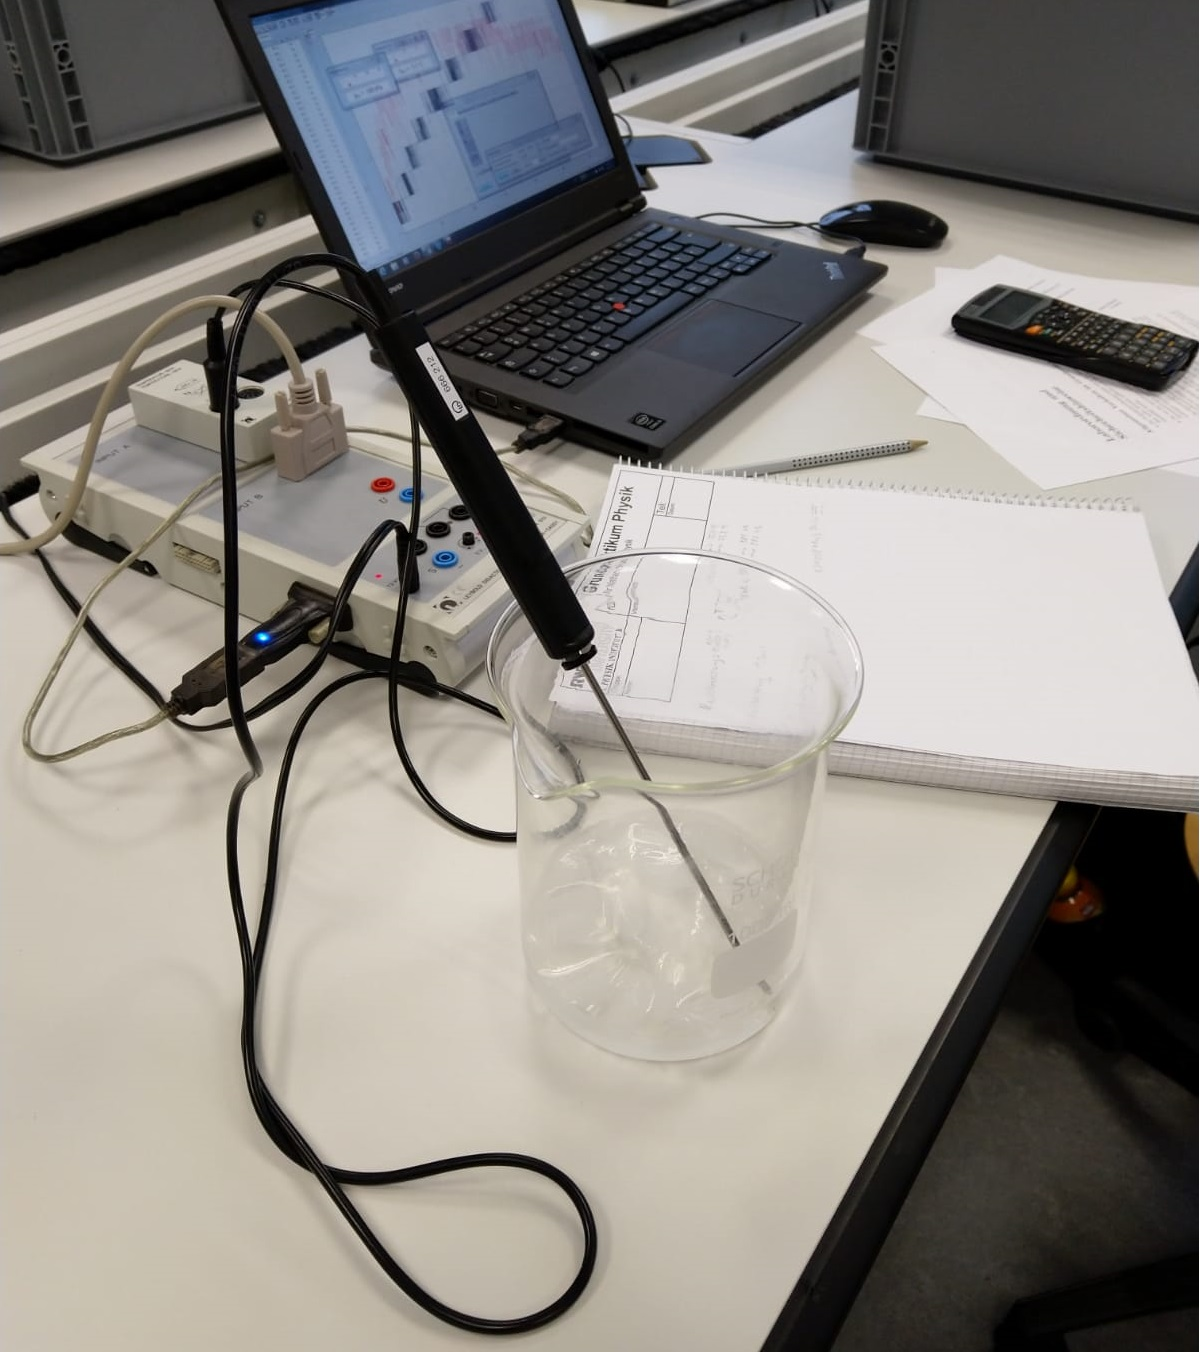
\includegraphics[scale=0.33]{Images/Cassy.jpg}
		\label{Cassy}
		\caption{Das verwendete Cassy-System samt Temperatur-Box und Druck-Input}
	\end{center}
\end{figure}
Versuchsdurchführung
Der Temperatursensor ist auf ein Intervall von \SI{-20}{\celsius} bis \SI{120}{\celsius} eingestellt, der Drucksensor auf ein Intervall von \SI{0}{\hecto\pascal}-\SI{1500}{\hecto\pascal}

\section{Durchführung}
\subsection{Rauschmessung}
Bei Raumtemperatur und Umgebungsdruck findet eine 'Leerlauf'-Messung statt, um den statistischen Fehler der Messgeräte gut abschätzen zu können. Dabei wird ein kurzes Zeitintervall bei hoher Messrate ausgewertet. 
Einstellungen: Messung alle 10ms, 16000 mal $\widehat{=}$ 3min

\subsection {Kalibrierung des Thermosensors}  {\color{red}[Sollen wir die Gasdichtigkeit vorziehen, um T0 und T100 in einem Punkt beschreiben zu können oder so tun, als wäre das Thermometerbei der Gasdichtigkeitsmessung im Kolben gewesen, und wir hätten davor T0 gemessen, weil am Aufbau nichts mehr verändert werden sollte?]}

Die Temperatur in Eiswasser wird zunächst gemessen, deren theoretischer Wert \SI{0}{\celsius} ist. Dazu wird Eis mit ein wenig Wasser gemischt und gewartet, bis ein Temperaturausgleich stattgefunden hat, der, solange noch festes Eis vorhanden ist, bei \SI{0}{\celsius} sein sollte, und die 7s Ansprechzeit, die der Sensor nach Angaben des Herstellers hat, verstrichen ist. Später, wenn das Wasser siedet, wird noch dessen Siedetemperatur bestimmt, die \SI{100}{\celsius} sein sollte. Mit einem linearen Modell kann man nun $T_{real}(T_{gemessen})$ bestimmen.
Einstellungen: Messung alle 100ms, insgesamt 3 Minuten lang.

\subsection{Gasdichtigkeit}
Um festzustellen, wie gasdicht der Aufbau ist, wird mit der Handpumpe im Kolben ein Unterdruck von etwa 190 hPa absolut erzeugt. Dann wird über einen Zeitraum von 10 Minuten der Druck gemessen, um hinterher mit Hilfe einer linearen Regression die Leckrate bestimmen zu können, die nicht höher sein sollte als 0.2 mbar/min {\color{red}[sollen wir 0.7 schreiben?]}, um zu gewährleisten, dass die gemessenen Druckwerte während der Hauptmessung nicht zu stark verfälscht werden. 
Einstellungen: Messung alle 100 ms, insgesamt 3 Minuten lang.


\subsection{Hauptmessung - Dampfdruckkurve}
Durch den zuvor erzeugten Unterdruck kann über den Dreiwegehahn Wasser in den Rundkolben gesaugt werden, bis dieser etwa halb voll ist. Mit Hilfe des Heizpilzes wird das Wasser bei Kontakt zur Umgebung zum Kochen gebracht und so lange kochen gelassen, bis der entstehende Wasserdampf sämtliche Restluft aus dem Rundkolben gedrückt hat. Dies prüft man, indem man den Verbindungsschlauch zur Umgebung in ein Wasserbad hält. Der Wasserdampf kondensiert sofort, das heißt, solange Blasen aufsteigen, befindet sich noch Luft im Rundkolben, deren Partialdruck die Messung verfälschen würde. In dieser Zeit wird auch die Kalibrierung bei \SI{100}{\celsius} durchgeführt. Schließlich wird der Heizpilz schnell mit dem Laborheber heruntergefahren und die Messung des Dampfdrucks und der Gastemperatur gestartet. Später sollen die Ergebnisse p und T in der Form $\ln(p/p_0)$ gegen $1/T-1/T_0$ aufgetragen werden, um aus der Steigung des Graphen $\Lambda$ zu bestimmen.
Einstellungen: Messung alle 100 ms, unbegrenzte Messdauer (Ende nach etwa einer Stunde)\\

\subsection{Gasdichtigkeit 2}

Nach der eigentlichen Versuchsdurchführung kann eine weitere Gasdichtigkeitsmessung wie 3. Durchgeführt werden, um zu gewährleisten, dass sich die Leckrate am Aufbau nicht verändert hat. Diese entfällt aber bei uns, da keine Zeit mehr ist.

\section{Auswertung}
{\color{red}- 7s Ansprechzeit?}\\
{\color{red}T100 wirklich 100 Grad bei unserem Druck?}\\
\subsection{Rauschmessung}
Die Rauschmessung umfasst 3326 Datenpunkte, bei denen der Temperatursensor in Ruhe die als konstant angenommene Raumtemperatur gemessen hat, der Absolutdrucksensor zugleich den konstanten Umgebungsdruck. Dabei soll die Streuung der Werte um den Mittelwert erarbeitet werden, um den statistischen Fehler für alle folgenden Messungen abschätzen zu können.\\
Die Ergebnisse sind wie folgt (Abb. \ref{RM_T} und \ref{RM_p}):\\
\begin{figure}[h]
	\begin{center}
		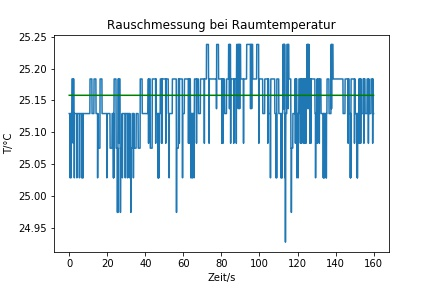
\includegraphics[scale=0.9]{Images/RauschmessungRT_T.jpg}
		\caption{Messergebnisse der Raumtemperatur-Rauschmessung}
		\label{RM_T}
	\end{center}
\end{figure}\\
\begin{figure}
	\begin{center}
			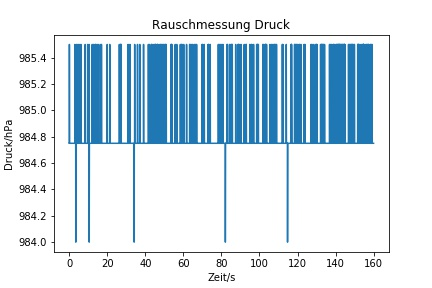
\includegraphics[scale=0.9]{Images/RauschmessungRT_p.jpg}
		\caption{Messergebnisse der Umgebungsdruck-Rauschmessung}
		\label{RM_p}
	\end{center}
\end{figure}
Die Temperaturmessung ergab einen Mittelwert von etwa \SI{25.1580}{\celsius} mit einer Standardabweichung von \SI{0.0444}{\celsius}. {\color{red}[Wie viele Nachkommastellen?]} Daraus ergibt sich ein statistischer Fehler von \SI{0.00077}{\celsius} (vgl. Abb.\ref{RM_T_histo}).\\
Die Druckmessung lieferte einen Mittelwert von 984.796 hPa mit einer Standardabweichung von 0.184 hPa und einem Fehler von 0.00319 hPa (vgl. Abb.\ref{RM_p_histo}).
\begin{figure}
	\begin{center}
		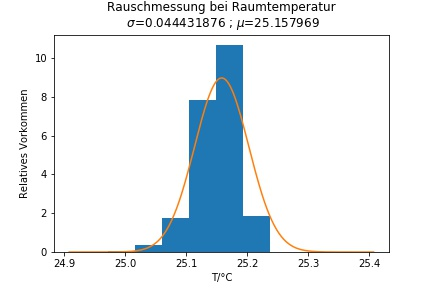
\includegraphics[scale=0.9]{Images/RauschmessungRT_T_histo.jpg}
		\caption{Histogramm der T-Rauschmessung}
		\label{RM_T_histo}
	\end{center}
\end{figure}
\begin{figure}
	\begin{center}
		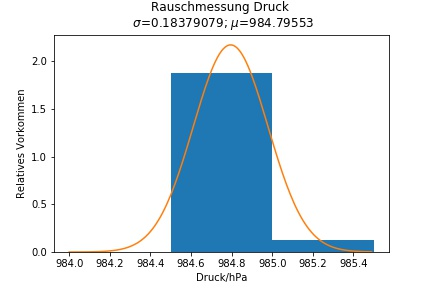
\includegraphics[scale=0.9]{Images/RauschmessungRT_p_histo.jpg}
		\caption{Histogramm der p-Rauschmessung}
		\label{RM_p_histo}
	\end{center}
\end{figure}
\end{document}
\subsection{Kalibrierung des Thermosensors}
Zur Kalibrierung des Thermometers wurde die Temperatur bei theoretischen \SI{0}{\celsius} und \SI{100}{\celsius} aufgezeichnet {\color{red}(vgl. Abb.)}.

